Под \vocab{параметрическим полиморфизмом} будем подразумевать возможность единообразно работать с произвольными типами данных.

В этом разделе мы рассмотрим различные классификации параметрически-полиморфных функций и техники связанные с ними.
Также немало внимания будет уделено обсуждению подходов к реализации параметрического полиморфизма в языках программирования.

\subsection{Параметрический полиморфизм в языке}

$\lambda$-абстракция позволяет обобщать выражения по значениям, каждая абстракция добавляет стрелку в тип выражения: $\lambda x\ldotp \lambda y\ldotp x : \alpha\to\beta\to\alpha$.
В то же время $\Lambda$-абстракция позволяет обобщать выражения по типам, добавляя квантор в тип: $\Lambda \alpha\ldotp\lambda x\ldotp \lambda y\ldotp x : \forall \alpha\ldotp \alpha\to\beta\to\alpha$.
Фактически такая функция теперь принимает три аргумента: тип и два значения.

Чтобы воспользоваться функцией, нужно в первую очередь специализировать её на нужный тип, передав его первым аргументом: $(\Lambda \alpha\ldotp\lambda x\ldotp \lambda y\ldotp x)\ap nat : nat\to\beta\to nat$.
Применение терма к типу называется \vocab{универсальной аппликацией}.

В Haskell большая $\Lambda$ приписывается неявно, однако есть экспериментальное расширение, позволяющее её писать --- \href{https://downloads.haskell.org/ghc/latest/docs/users_guide/exts/type_abstractions.html}{TypeAbstractions}.
\mintinline{haskell}|forall| тоже обычно неявно приписываются к типам, связывая, по конвенции, все типы, начинающиеся с маленькой буквы в порядке их вхождения в тип.
Однако у пользователя есть возможность явно приписывать \mintinline{haskell}|forall|'ы с помощью расширения \href{https://downloads.haskell.org/ghc/latest/docs/users_guide/exts/explicit_forall.html\#extension-ExplicitForAll}{ExplicitForAll}.
Это может понадобиться либо за тем, чтобы изменить порядок автоматических типовых абстракций, либо чтобы иметь возможность сослаться на абстрагированный тип в теле функции (расширение \href{https://downloads.haskell.org/ghc/latest/docs/users_guide/exts/scoped_type_variables.html#extension-ScopedTypeVariables}{ScopedTypeVariables}).

Haskell также позволяет вручную прописывать типовые аппликации (с помощью расширения \href{https://downloads.haskell.org/ghc/latest/docs/users_guide/exts/type_applications.html}{TypeApplications}).
Это может помочь программированию на уровне типов, когда информации из терма не достаточно, чтобы специализировать тип.
\begin{minted}{haskell}
    id :: forall a . a -> a
    ghci> :t id @Int
    id @Int :: Int -> Int
\end{minted}

Конструкторы данных формально описываются путём использования лямбда-абстракций и редукций на уровне типов.
Таким образом, возникает необходимость контроля за корректностью типовых аппликаций, которая осуществляется системой кайндов.
\begin{align*}
    &Pair : * \rightarrow * \rightarrow * \\
    &Pair = \lambda \tau^*~\sigma^*\ldotp\forall \gamma\ldotp(\tau\rightarrow\sigma\rightarrow\gamma)\to\gamma \\
    &pair : \forall \alpha~\beta\ldotp\alpha \rightarrow \beta \rightarrow Pair~\alpha~\beta \\
    &pair = \Lambda \alpha^*~\beta^*\ldotp\lambda x^\alpha~y^\beta\ldotp(\Lambda \gamma^*\ldotp\lambda f^{\alpha\rightarrow\beta\rightarrow\gamma}\ldotp f~x~y) \\
    &fst : \forall \alpha~\beta\ldotp Pair~\alpha~\beta\rightarrow \alpha \\
    &fst = \Lambda \alpha^*~\beta^*\ldotp\lambda p^{Pair~\alpha~\beta}\ldotp p~\alpha~(\mathbf{K}\ap\alpha\ap\beta)
\end{align*}

Haskell не позволяет создавать функции на типах по месту с помощью явной типовой лямбды\footnote{\url{https://stackoverflow.com/questions/4069840/lambda-for-type-expressions-in-haskell}}.
В Scala существует нетривиальный трюк\footnote{\href{https://stackoverflow.com/questions/8736164/what-are-type-lambdas-in-scala-and-what-are-their-benefits}{(stackoverflow) Scala type lambdas.}}\footnote{https://stackoverflow.com/questions/9443004/what-does-the-operator-mean-in-scala}, который позволяет этого добиться.
Scala3, однако, включила эту возможность непосредственно в язык\footnote{\url{https://docs.scala-lang.org/scala3/reference/new-types/type-lambdas.html}}.

\subsubsection{First-class polymorphism}

Существует возможность писать функции, которые принимают другие полиморфные функции в качестве аргументов.
Типы таких функций называются \vocab{типами высшего ранга (higher-ranked types)}, их можно использовать с расширением \href{https://downloads.haskell.org/ghc/latest/docs/users_guide/exts/rank_polymorphism.html}{RankNTypes}.
Так, типовой параметр функции \texttt{g} определяет функция \texttt{f}, а не вызывающий функцию \texttt{f}:
\begin{minted}{haskell}
    f :: (forall a . a -> a) -> (Int, Char)
    f g = (g @Int 42, g @Char 'a') -- универсальная аппликация для наглядности
    ghci> f (\x -> x)
\end{minted}

Проблема типов высшего ранга в том, что их вывод неразрешим, то есть глобальный вывод типов Haskell в этом случае перестаёт работать.
Но если типы высшего ранга приписать вручную, остальной вывод будет работать как и раньше.
Например, числа Чёрча имеют высший ранг\footnote{\url{https://okmij.org/ftp/tagless-final/course/Boehm-Berarducci.html}}:
\begin{minted}{haskell}
    suc :: (forall a . (a -> a) -> a -> a) -> (a -> a) -> a -> a
    suc n s z = s (n s z)
\end{minted}

%! suppress = LineBreak
\begin{task}
    Какой ранг имеет тип тип \mintinline{haskell}|Int -> (forall a . a -> a)|?
\end{task}

По умолчанию типовые параметры можно специализировать только на конкретные типы.
Расширение \href{https://downloads.haskell.org/ghc/latest/docs/users_guide/exts/impredicative_types.html}{ImpredicativeTypes} позволяет специализировать типовые параметры на полиморфные типы (включающие \mintinline{haskell}|forall|'ы внутри себя) --- \vocab{импредикативное применение}.
\begin{minted}{haskell}
    runST :: (forall s. ST s a) -> a
    id :: forall b. b -> b
    foo = id runST -- типизируется только с ImpredicativeTypes
\end{minted}

Типы высших рангов вместе с импредикативным применением образуют \vocab{полиморфизм первого класса (first-class polymorphism)}, когда полиморфные типы могут использоваться почти так же свободно, как и любые другие.
Классический алгоритм вывода Хиндли-Дамаса-Милнера не справляется (и в общем случае задача неразрешима), так что существует большое количество решений, делающих различные компромиссы.
Наиболее известные --- FreezeML~\cite{emrich2020freezeml} и Quick Look\footnote{\href{https://youtu.be/ZuNMo136QqI?si=qp8PAEeeF-bioCB_}{(youtube) A Quick Look at Impredicativity (Simon Peyton Jones)}}~\cite{serrano2020quick}, реализованный в Haskell с недавнего времени.

\subsubsection{Higher-kinded polymorphism}

Haskell позволяет также абстрагироваться по типам произвольных кайндов, не только \mintinline{haskell}|Type|.
Например, \mintinline{haskell}|f :: forall (m :: Type -> Type) a . a -> m a|.

% todo too polymorphic: theorems for free

Говорят, что функции, возвращающие значение какого-то такого вида \texttt{m a} --- слишком полиморфные, ``too polymorphic''.
Код, использующий такие функции будет сталкиваться с серьёзнами проблемами в производительности, так как компилятор не знает конкретного типа и не может заинлайнить соответствующие вызовы \texttt{fmap}, bind, и т.д.
Чтобы обойти эту проблему, рекомендуется пользоваться либо конкретными типами, либо воспользоваться библиотекой kan-extensions\footnote{\url{https://hackage.haskell.org/package/kan-extensions}}\footnote{\url{https://bartoszmilewski.com/2017/04/17/kan-extensions/}}~\cite[параграф 13.5]{maguire-types}.

Далеко не во всех языках есть полиморфизм высшего ранга, но иногда он нужен.
Например, если мы хотим объявить абстрактный тип \mintinline{haskell}|Monad|.
Заметим, что тип кайнда \mintinline{haskell}|Type -> Type| --- это функция на типах, принимающая один тип, и возвращающая другой.
Соответственно, функция, абстрагированная по такому типу~--- функция высшего порядка, в некотором смысле.
Но мы уже знаем технику избавления от них --- дефункцинализация~\cite{defunctionalization-slides}.
Рассмотрим пример на языке Kotlin.

Будем представлять типовую аппликацию в виде отдельного типа \mintinline{kotlin}|Apply<Sym, T>|.
Установим изоморфизм между \mintinline{kotlin}|List<T>| и \mintinline{kotlin}|Apply<ListSym, T>|:
\begin{minted}{kotlin}
    class Apply<Sym, T>(val value: Any)
    object ListSym

    fun <T> List<T>.to(): Apply<ListSym, T> = Apply(this)
    fun <T> Apply<ListSym, T>.from(): List<T> = this.value as List<T>
\end{minted}

Теперь мы можем объявить интерфейс монад и задать реализацию для списка с помощью синглтона:
\begin{minted}{kotlin}
    interface Monad<M> {
        fun <T> pure(x: T): Apply<M, T>
        infix fun <T, R> Apply<M, T>.bind(k: (T) -> Apply<M, R>): Apply<M, R>
    }

    object ListMonad : Monad<ListSym> {
        override fun <T> pure(x: T): Apply<ListSym, T> = listOf(x).to()
        override fun <T, R> Apply<ListSym, T>.
                bind(k: (T) -> Apply<ListSym, R>): Apply<ListSym, R> =
            this.from().flatMap { k(it).from() }.to()
    }
\end{minted}

И наконец мы можем писать функции над произвольными монадами:
\begin{minted}{haskell}
    fun <M> Monad<M>.go(x: Apply<M, Int>): Apply<M, Int> =
        x bind { pure(it + 1) } bind { pure(it + 2) }

    fun test(xs: List<Int>): List<Int> = ListMonad.go(xs.to()).from()
\end{minted}

Не лишним будет отметить, что результирующий код выглядит несколько чудовищно.
Скорее всего, использование этой техники не окупает себя и нужно выбирать другой стиль программирования.
Однако иметь этот инструмент в ящике не будет лишним.

\subsubsection{Вариантность}

В этом параграфе мы будем рассматривать тему с точки зрения программирования~\cite[глава 3]{maguire-types}, не отдавая должного теории категорий.
Восполнить пробел можно с помощью замечательной статьи, написанной в жанре пьесы~\cite{hinze2012functional}.

\vocab{Ковариантный функтор} --- пара из типового конструктора \texttt{F} и операции на функциях \texttt{fmap :: (a -> b) -> (F a -> F b)}.
Плюс законы о том, что \texttt{fmap} уважает \texttt{id} и композицию.

\begin{minted}{haskell}
    class Functor f where
      fmap :: (a -> b) -> (f a -> f b)
\end{minted}

\begin{figure}[H]
    \centering
    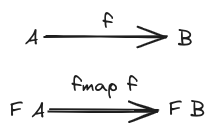
\includegraphics[width=0.3\textwidth]{figs/functor}
\end{figure}

\vocab{Контравариантный функтор} --- пара из типового конструктора и операции на функциях, разворачивающей стрелку.
Плюс соответствующие законы.

\begin{minted}{haskell}
    class Contravariant f where
      contramap :: (a -> b) -> (f b -> f a)
\end{minted}

\begin{figure}[H]
    \centering
    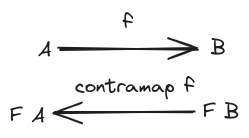
\includegraphics[width=0.3\textwidth]{figs/contra-functor}
\end{figure}

Типовой конструктор можно объявить ковариантным или контравариантным функтором (или никаким из них) относительно типового параметра в зависимости от вида декларации соответствующих конструкторов данных.
А именно, от \vocab{полярности}\footnote{\url{https://existentialtype.wordpress.com/2012/08/25/polarity-in-type-theory/}}\footnote{\url{https://ncatlab.org/nlab/show/polarity+in+type+theory}} позиций, в которых входит этот типовой параметр в декларации.

Попробуем развить интуитивное понимание полярностей.
Рассмотрим некоторое вычисление типа \texttt{F a}.
Параметр \texttt{a} входит в положительной позиции, если все его значения можно извлечь из \texttt{F a}, как в следующих примерах (для извлечения могут понадобиться паттерн-матчинг и аппликация):
\begin{minted}{haskell}
    data F a = L a | R a
    data F a = D a (Int -> a)
\end{minted}

Вхождения, наоборот, отрицательные, если значения соответствующего типа нельзя получить из вычисления, но нужно ему предоставить.
Например, в качестве параметров функций:
\begin{minted}{haskell}
    data F a = F (a -> Int)
    data F a = L (a -> ()) | R Int
\end{minted}
Действительно, для первого примера можно объявить инстанс \mintinline{haskell}|Contravariant|:
\begin{minted}{haskell}
    instance Contravariant F where
      contramap :: (a -> b) -> (F b -> F a)
      contramap g (F f) = F (f . g)
\end{minted}

Можно предположить, что на плюс и минус действуют обычные мультипликативные законы.
И это действительно так.
\begin{itemize}
    \item Плюс на плюс даёт плюс:
    \begin{minted}{haskell}
        data F a = F (Int -> (Int -> a))
    \end{minted}
    \item Плюс на минус (и наоборот) --- минус:
    \begin{minted}{haskell}
        data F a = F ((Int -> a) -> Int)
    \end{minted}
    \item Минус на минус --- плюс, поскольку параметр принимаемой функции выдаётся реализацией вызывающей стороне:
    \begin{minted}{haskell}
        data F a = F ((a -> Int) -> Int)
    \end{minted}
\end{itemize}

Тип от двух положительных параметров можно объявить \vocab{бифунктором}:
\begin{minted}{haskell}
    class Bifunctor f where
      bimap :: (a -> c) -> (b -> d) -> f a b -> f c d
\end{minted}

Тип от двух параметров, положительного и отрицательного, --- \vocab{профунктором}:
\begin{minted}{haskell}
    class Profunctor p where
      dimap :: (c -> a) -> (b -> d) -> p a b -> p c d
\end{minted}

Профункторы являются некоторыми обобщениями функциональной стрелки.
Например, если у нас есть SQL запрос, который по данным возвращает результат, его можно объявить профунктором с семантикой --- добавить пред-обработку входных данных и пост-обработку выходных:
\begin{minted}{haskell}
    dimap serialize deserialize (query :: Text -> Text) :: Age -> [User]
\end{minted}

Также понятие вариантности часто встречается в объектно ориентированных языках для обозначения возможности дополнить отношение подтипизации на полиморфные типы (да и вообще в теории подтипизации).

Действительно, \vocab{отношение подтипизации} \texttt{B <: A} говорит о том, что значение типа \texttt{B} безопасно использовать в позиции, где ожидается значение типа \texttt{A}.
Иначе говоря, существует функция \texttt{upcast :: B -> A}.
Если типовой конструктор \texttt{F a} ковариантен относительно параметра \texttt{a}, то по \texttt{upcast} найдётся \texttt{upcast' :: F B -> F A}.
То есть отношение подтипизации также автоматически включает \texttt{F B <: F A}.
Контравариантный случай аналогично.

\begin{task}
    Убедитесь в вашем любимом языке с поддержкой вариантности, что минус на минус даёт плюс.
\end{task}

\subsubsection{Data promotion \& kind polymorphism} \label{subsubsec:promotion}

Ранее мы программировали на уровне термов, а типы контролировали ``правильность'' построения термов.
Но типы так же являются языком как с синтаксической точки зрения, так и с вычислительной.
Вычисления на типах мы будем рассматривать далее, а в этом параграфе научимся конструировать в Haskell различные структуры на уровне типов.

В качестве модельной задачи зададим структуру данных, моделирующую вектор, но такую, что тип будет параметризован длиной.
Для начала определим натуральные числа на уровне типов в стиле Пеано:
\begin{minted}{haskell}
    data Zero
    data Suc n
\end{minted}

\begin{task}
    Сколько обитателей типа \mintinline{haskell}|Suc (Suc Zero)|?
\end{task}

Теперь мы можем задать тип вектора, содержащий информацию о длине:
\begin{minted}{haskell}
    data Vec (size :: Type) (elem :: Type) where
      VNil :: Vec Zero a
      VCons :: a -> Vec n a -> Vec (Suc n) a

    example :: Vec (Suc (Suc Zero)) Int
    example = VCons 1 (VCons 2 VNil)
\end{minted}

Для такого типа, например, можно написать безопасную функцию \mintinline{haskell}|zip|, работающую только на векторах одинаковой длины:
\begin{minted}{haskell}
    vzip :: Vec n a -> Vec n b -> Vec n (a, b)
    vzip VNil VNil = VNil                                      -- n ?$\sim$? Zero
    vzip (VCons x xs) (VCons y ys) = VCons (x, y) (vzip xs ys) -- n ?$\sim$? Suc n'
\end{minted}

Заметьте, что в остальных ветках \mintinline{haskell}|vzip| должны возникнуть эквивалентности, начинающиеся с различных конструкторов, например, \mintinline{haskell}|Zero ?$\sim$? Suc n|.
Поскольку невозможно построить такие аргументы функции, Haskell позволяет соответствующие ветки не рассматривать.

\begin{task}
    Напишите функцию добавления в конец элемента вектора.
    Двигайтесь последовательно, заполняя типовые дыры и отслеживая возникающие эквивалентности.
\end{task}

Удивительно, но сейчас наш язык типов не типизирован.
Действительно, кайнд \mintinline{haskell}|Suc| --- \mintinline{haskell}|Suc :: Type -> Type|, соответственно ничто не мешает написать \mintinline{haskell}|Suc (Maybe Int)|.
То есть язык кайндов, который должен контролировать типы, слишком беден.
В то же время он слишком ограничивающий, поскольку не поддерживает полиморфизм, что дало начало большому количеству дублирований а ля \mintinline{haskell}|Typeable (ty :: Type)|, \mintinline{haskell}|Typeable1 (ty :: Type -> Type)|\ldots

Чтобы обогатить систему кайндов для лучшего контроля за программами уровня типов, System $F_C$ была расширена до System $F_C^\uparrow$ (читается FC-pro)~\cite{yorgey2012giving}.
Это достигается автоматическим продвижением (promotion) \mintinline{haskell}|data| деклараций на уровень выше (расширение \href{https://downloads.haskell.org/ghc/latest/docs/users_guide/exts/data_kinds.html#extension-DataKinds}{DataKinds}).
А именно: любой конструктор типа также становится кайндом, а конструктор данных --- конструктором типа.
Так, в примере с числами, мы можем задекларировать натуральные числа как обычно и использовать на уровне типов:
\begin{minted}{haskell}
    data Nat = Zero | Suc Nat
    ghci> :k Suc :: Nat -> Nat
\end{minted}

Теперь вектору можно приписать более точный кайнд:
\begin{minted}{haskell}
    data Vec (size :: Nat) (elem :: Type) where
      VNil :: Vec Zero a
      VCons :: a -> Vec n a -> Vec (Suc n) a
\end{minted}

\begin{task}
    Что выведет \mintinline{haskell}|ghci> :k Vec|?
\end{task}

Поскольку типы и термы в Haskell живут в разных пространствах имён, можно называть конструкторы типов и данных одинаково.
Однако если продвинуть такой тип данных, возникнет неоднозначность: мы имеем в виду тип или продвинутый конструктор.
Haskell позволяет указать явно, что речь идёт о продвинутом конструкторе с помощью одинарной кавычки.
\begin{minted}{haskell}
    data T = T Nat
    ghci> :k T
    T :: Type      -- Речь про конструктор типа
    ghci> :k 'T
    'T :: Nat -> T -- Речь про продвинутый конструктор данных
\end{minted}

Недавние версии GHC поддерживают прямое объявление конструкций уровня типов с помощью расширения \href{https://downloads.haskell.org/ghc/latest/docs/users_guide/exts/type_data.html#extension-TypeData}{TypeData}.
Не любые \mintinline{haskell}|data| декларации подходят для продвижения, в то же время \mintinline{haskell}|type data| декларации позволяют явно запросить структуру уровня типов и получить внятные ошибки, если декларация написана неправильно.
\begin{minted}{haskell}
    type data Nat = Zero | Suc Nat
\end{minted}

В случае продвижения полиморфного типа, мы получаем полиморфные кайнды (\href{https://downloads.haskell.org/ghc/latest/docs/users_guide/exts/poly_kinds.html}{PolyKinds}):
\begin{minted}{haskell}
    data [a] = [] | (:) a [a]
    ghci> :k '(:)
    '(:) :: forall k . k -> [k] -> [k]
\end{minted}

\begin{figure}
    \centering
    %! suppress = Quote
    \begin{tabular}{|c|c|c|}
        \hline
        Term                                   & Type                                            & Kind                                            \\
        \hline
        \mintinline{haskell}|Zero|             & \mintinline{haskell}|Nat|                       & \mintinline{haskell}|Type|                      \\
        \mintinline{haskell}|[Zero, Suc Zero]| & \mintinline{haskell}|[Nat]|                     & \mintinline{haskell}|Type|                      \\
        \mintinline{haskell}|[]|               & \mintinline{haskell}|forall a. [a]|             & \mintinline{haskell}|Type|                      \\
        \mintinline{haskell}|(:)|              & \mintinline{haskell}|forall a. a -> [a] -> [a]| & \mintinline{haskell}|Type|                      \\
        & \mintinline{haskell}|'Suc 'Zero|                & \mintinline{haskell}|Nat|                       \\
        & \mintinline{haskell}|'['Zero, 'Suc 'Zero]|      & \mintinline{haskell}|[Nat]|                     \\
        & \mintinline{haskell}|'[Int, Double]|            & \mintinline{haskell}|[Type]|                    \\
        & \mintinline{haskell}|'[]|                       & \mintinline{haskell}|forall k. [k]|             \\
        & \mintinline{haskell}|'(:)|                      & \mintinline{haskell}|forall k. k -> [k] -> [k]| \\
        \hline
    \end{tabular}
    \caption{Пример продвижений в Haskell.}
    \label{fig:universes}
\end{figure}

Примеры продвижения различных конструкций можно увидеть в таблице~\ref{fig:universes}.

Зададим гетерогенный список, индексированный типами элементов:
\begin{minted}{haskell}
    data HList (tys :: [Type]) where
      HNil :: HList '[]
      HCons :: ty -> HList tys -> HList (ty ': tys)

    example :: HList '[Int, Bool, Double]
    example = HCons 42 $ HCons True $ HCons 12.5 HNil
\end{minted}

Структуры данных тоже могут быть полиморфными по кайндам.
Рассмотрим следующий тип \href{https://hackage.haskell.org/package/tagged-0.8.8/docs/Data-Tagged.html#t:Tagged}{\mintinline{haskell}|Tagged|}, позволяющий дополнить тип значения дополнительным типовым тегом.
Кайнд тега может быть произвольным, поэтому, например, можем использовать встроенные в систему типов константы \href{https://ghc.gitlab.haskell.org/ghc/doc/users_guide/exts/type_literals.html}{TypeLits}:
\begin{minted}{haskell}
    newtype Tagged (tag :: k) (a :: Type) = Tagged a
    ghci> :t Tagged
    Tagged :: forall k (tag :: k) a. a -> Tagged tag a

    example :: Tagged ("hello" :: Symbol) Int
    example = Tagged 42
\end{minted}

Современный Haskell в итоге пришёл к тому, что система типов не делает различий между типами и кайндами (рис.~\ref{fig:types-eq-kinds}).
В частности, \mintinline{haskell}|Type :: Type|.
Это нужно для расширения возможностей Haskell в сторону программирования с зависимыми типами путём добавления несинтаксических эквивалентностей для кайндов (\href{https://ghc.gitlab.haskell.org/ghc/doc/users_guide/exts/poly_kinds.html#extension-TypeInType}{TypeInType}).
$System~FC$ была представлена в работе~\cite{weirich2013system}\footnote{\href{https://www.youtube.com/watch?v=ISGENChlA4M&list=PLvPsfYrGz3wufQguebnCduYgQQ9UMeJRt}{(youtube) Мини-курс на русском языке про развитие Haskell в сторону зависимой типизации.}}\footnote{\href{https://www.youtube.com/watch?v=_HYI7zjkrEs&list=PLvPsfYrGz3wuVAGhNf6-i7uafXg56oqM5&index=1}{(youtube) Мини-курс на русском языке --- система вывода типов Haskell.}}.

\begin{figure}
    \centering
    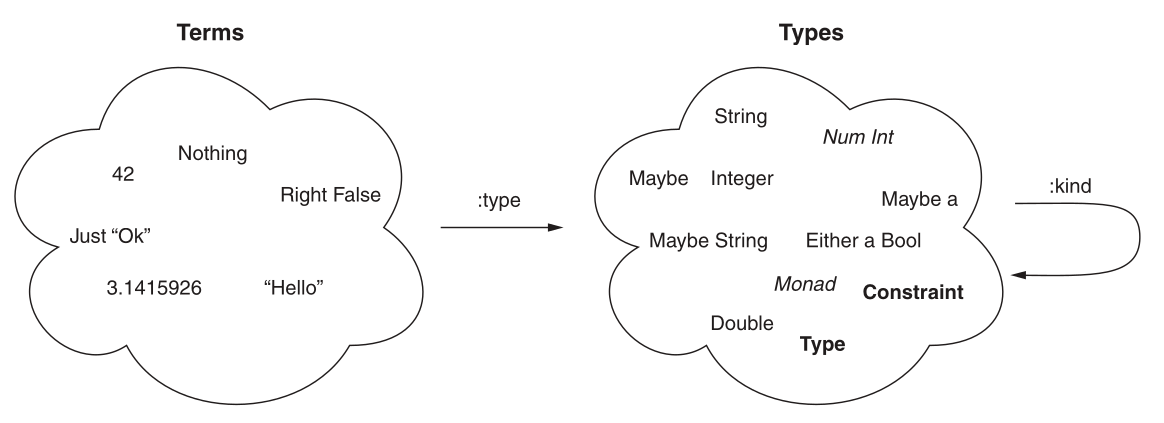
\includegraphics[width=0.99\textwidth]{figs/types-eq-kinds}
    \caption{Типы и канды --- одно~\cite{bragilevsky-haskell}.}
    \label{fig:types-eq-kinds}
\end{figure}

\subsection{Реализация параметрического полиморфизма}

\vocab{Конвенция вызова}\footnote{\url{https://en.wikipedia.org/wiki/Calling_convention}} представляет собой набор соглашений между тем, как функция компилируется и как должна вызываться.
Например, функция принимает два аргумента, каждый размером в машинное слово, и возвращает один результат размером в машинное слово.
Тогда сгенерированный низкоуровневый код этой функции может, например, ожидать, что оба аргумента передаются через специальную пару регистров, а складывать результат он будет в третий.
В таком случае вызывающий код обязан предоставить аргументы в правильных регистрах и ожидать результата в некотором третьем, заранее оговоренном регистре.

В общем случае, конвенция вызова функции зависит от типов аргументов и результата.
Нужно знать как минимум их размер, чтобы понять, размещать их в регистрах или на стеке.
Нужно знать, это указатель или значение само по себе, чтобы понимать, как с ним работать.

Таким образом, реализация параметрического полиморфизма в языке --- это не тривиальная задача.
Разные языки используют различные подходы, все со своими достоинствами и недостатками.

\subsubsection{Mономорфизация} \label{subsubsec:monomorphization}

\vocab{Mономорфизация} --- самый прямолинейный подход, компилируем функцию отдельно для каждого набора типовых аргументов.
Так, если различных наборов типовых аргументов, с которыми эта функция вызывается, например, 100 (что запросто может быть), то её код будет компилироваться сто раз и занимать в бинарнике в сто раз больше места.
Так делают, например, C++ и Rust.

На самом деле всё ещё хуже.
Если проект многомодульный и состоит из множества единиц компиляции (кусков, которые компилируются отдельно), то одна и та же специализация функции на типовые аргументы будет компилироваться заново во всех единицах компиляции, где такая специализация нужна.
А затем, линкер будет заниматься удалением дубликатов, что тоже не самый быстрый и эффективный процесс.

\begin{itemize}
    \item[\positive] Порождаемый код максимально эффективен для каждого типа;
    \item[\negative] Время компиляции крайне велико;
    \item[\negative] Существенно увеличивается размер результирующего бинарного файла, что может быть критично для некоторых приложений;
    \item[\negative] Может неэффективно работать из-за засорения кеша кода в процессоре;
    \item[\negative] В интерфейсах не может быть полиморфных методов, так как мы не знаем в месте вызова, к какому именно наследнику относится вызываемый метод, и какой код нужно специализировать;
    \item[\negative] К полиморфным функциям нельзя динамически линковаться (у них нет кода до специализации);
    \item[\negative] Нельзя поддержать variance, потому что код компилируется для конкретного типа и в общем случае не может работать для произвольного подтипа или супертипа.
\end{itemize}

Некоторые языки не делают инстанциацию скрытой деталью реализации языка, а предоставляют её как инструмент пользователям.
Так делают, например, C++ и Zig.
А именно, это позволяет добиться следующего:
\begin{itemize}
    \item Если разрешить использовать значения в типах, инстанциация может использоваться как механизм вычислений на этапе компиляции.
    \item Если отложить проверку ошибок на стадию инстанциирования, то мы получим своего рода статическую утиную типизацию.
    Это позволит не описывать сложные сигнатуры полиморфных функций.
    Однако тогда функции придётся вручную инстанциировать против всевозможных типов, иначе нельзя понять статически, компилируется она хотя бы против этих типов или нет.
\end{itemize}

\subsubsection{Стирание типа} \label{subsubsec:type-erasure}

Можно всё сделать наоборот, унифицировав значения, которые приходят на вход полиморфным функциям, вместо того, чтобы компилировать код под каждый тип.

Пусть каждое значение будет аллоцировано в куче и передаваться по указателю.
Тогда мы сможем переиспользовать один и тот же код для разных типовых аргументов, он просто будет ожидать указатели.

\begin{itemize}
    \item[\positive] Каждая функция компилируется ровно один раз --- быстро;
    \item[\positive] Можно динамически загружать новые полиморфные функции и типы и использовать их друг с другом;
    \item[\positive] Гибкость --- вариантность, полиморфные методы в интерфейсах, higher-ranked types\ldots просто работают;
    \item[\negative] Аллокация в куче и разыменование указателя может очень сильно замедлить код, особенно работающий с ``примитивными типами'';
    \item[\negative] Поскольку информация о типах стирается, нельзя ничего сделать с типовым аргументом, не имея его обитателей (например, запросить рефлексией информацию).
\end{itemize}

Такого подхода придерживаются JVM, Haskell и, как правило, другие функциональные языки ввиду его гибкости.

Особую проблему вызывает работа с примитивами, потому что каждое значение приходится сначала боксить (переносить в кучу), а потом уже использовать в полиморфном контексте.
Поэтому языки борются с этим как могут.
Некоторые языки урезают диапазоны значений примитивов, чтобы зарезервировать бит, определяющий, это указатель или значение.
Код консультируется с этим битом для работы (похоже на~\ref{subsubsec:swift-generics}).
Так делают, например, OCaml и \href{https://koka-lang.github.io/koka/doc/book.html#sec-value-types}{Koka}.
Агрессивный инлайнинг тоже помогает.
Java пытается аккуратно двигаться в сторону возможности мономорфизации\footnote{\href{https://youtu.be/JI09cs2yUgY?si=MLkRs31mN1koXIu1}{Type Specialization of Java Generics - What If Casts Have Teeth ?}}\footnote{\url{https://cr.openjdk.org/~jrose/values/parametric-vm.html}}.

\subsubsection{Гибридный подход} \label{subsubsec:hybrid}

С\# реализует гибридный подход\footnote{\href{https://learn.microsoft.com/en-us/dotnet/csharp/programming-guide/generics/generics-in-the-run-time}{Generics in the runtime (C\# programming guide).}}.
Они различают значения, хранимые в куче --- \vocab{reference types}, и значения, хранимые на стеке --- \vocab{value types}.
Для первых они генерируют одну специализацию, работающую с указателями.
Для каждого набора value-типов они генерируют лениво в рантайме специализацию.

То есть следы дженериков в таком подходе есть в промежуточном представлении CIL, а также в рантайме.

\begin{itemize}
    \item[\positive] Порождается эффективный код, работающий с примитивами;
    \item[\positive] Доступна рефлексия по дженерикам;
    \item[\positive] Небольшое время компиляции;
    \item[\negative] Инстанциация в рантайме замедляет исполнение;
    \item[\negative] Variance работает только для reference types (что странно --- есть ``правильная'' подтипизация, а есть ``неправильная'').
\end{itemize}

% todo выпросить инфу про подтипизацию у Михаила

\subsubsection{Использование виртуальной таблицы свойств типов} \label{subsubsec:swift-generics}

Swift\footnote{\href{https://youtu.be/ctS8FzqcRug?si=y_ZYnuUOulA33d_X}{2017 LLVM Developers’ Meeting: ``Implementing Swift Generics''}} вместе с каждым типовым параметром передаёт value witness table (рис.~\ref{fig:swift-witness-table}).
Это таблица со всей необходимой информацией, о типе: размер и выравнивание, что нужно сделать при копировании и перемещении объекта (например, инкрементировать счётчик ссылок).
Таким образом, скомпилированный код постоянно обращается к этой таблице и делает виртуальные вызовы функций из неё (рис.~\ref{fig:swift-generated-code}).
\begin{figure}
    \centering
    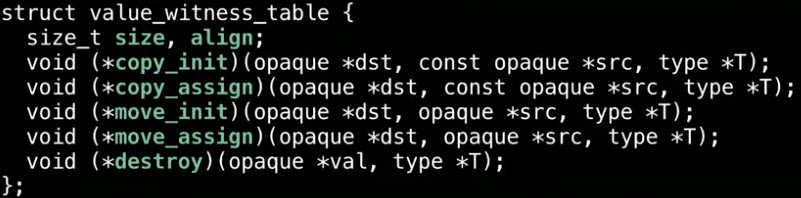
\includegraphics[width=0.7\textwidth]{figs/swift-witness-table}
    \caption{Swift value witness table.}
    \label{fig:swift-witness-table}
\end{figure}
\begin{figure}
    \centering
    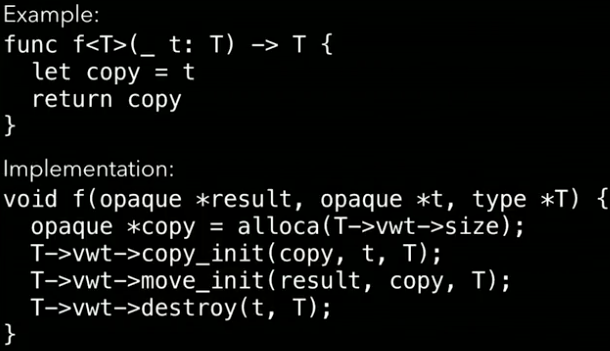
\includegraphics[width=0.6\textwidth]{figs/swift-generated-code}
    \caption{Код полиморфной функции, порождаемый компилятором Swift.}
    \label{fig:swift-generated-code}
\end{figure}

\begin{itemize}
    \item[\positive] Небольшое время компиляции;
    \item[\positive] Предсказуемая эффективность (не приводит к неожиданным паузам в рантайме);
    \item[\positive] Эффективная работа с value-значениями;
    \item[\positive] Высокая гибкость;
    \item[\positive] Информация о типах не стирается;
    \item[\negative] Серьёзный константный оверхед на динамические вызовы через таблицу, эффективность очень сильно зависит от компиляторных оптимизаций.
\end{itemize}

Своего рода реализация параметрического полиморфизма через специальный.

\subsection{Полиморфизм по конвенции вызова} \label{subsec:representation-polymorphism}

Как мы уже обсуждали выше~\ref{subsubsec:type-erasure}, параметрический полиморфизм в Haskell реализуется следующим образом: все значения хранятся в куче и передаются в полиморфные функции по указателю.
Однако, если для вычислительного кода важна производительность, такой подход не годится ввиду большой нагрузки на подсистему управления памятью и множества индирекций.
Поэтому Haskell позволяет также писать код с использованием unboxed значений.
А если конвенция вызова не принципиальна, можно по ней абстрагироваться и писать один код для boxed и unboxed значений~\cite{eisenberg2017levity}.

\subsubsection{Классификация значений по runtime представлению}

\begin{figure}
    \centering
    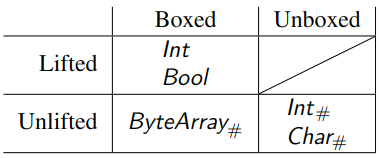
\includegraphics[width=0.5\textwidth]{figs/haskell-value-kinds}
    \caption{Виды значений в Haskell с примерами~\cite{eisenberg2017levity}.}
    \label{fig:haskell-value-kinds}
\end{figure}

На рисунке~\ref{fig:haskell-value-kinds} можно увидеть классификацию значений в Haskell с примерами типов.
\vocab{Unboxed типы} --- их значения удерживаются и передаются по значению.
\vocab{Boxed}, соответственно, наоборот, передаются по указателю и хранятся в куче.
Обычный \mintinline{haskell}|Int| является просто декларацией следующего вида, где \mintinline{haskell}|I#| --- это обычный конструктор с необычным именем, содержащий unboxed значение.
\begin{minted}{haskell}
    data Int = I# Int#
\end{minted}

\vocab{Lifted типы} --- содержат $\bot$ в качестве значения.
Иначе говоря, могут содержать отложенные вычисления.
\vocab{Unlifted типы} --- наоборот, не могут быть отложенными.
Операции, производящие значения unlifted типов всегда энергичные.
Свойство lifted/unlifted называют \vocab{levity}.
Чтобы распространить дальнейшее изложение на энергичные языки, можно levity заменить на boxity и всё останется справедливым.

\# в именах типов и функций --- это конвенция, показывающая, что где-то рядом происходит работа с unlifted значениями\footnote{Нужно подключить расширение \href{https://ghc.gitlab.haskell.org/ghc/doc/users_guide/exts/magic_hash.html}{MagicHash}, чтобы пользоваться \# в идентификаторах.}.

Также в Haskell есть unboxed кортежи, которых не существует на этапе исполнения.
Например, следующая функция как бы возвращает пару значений, но в действительности компилятор может их разместить, например, в паре регистров.
Соответственно, паттерн-матчинг по таким кортежам, просто позволяет сослаться на каждое из этих значений.
\begin{minted}{haskell}
    divMod# :: Int -> Int -> (# Int, Int #)
    case divMod# n k of (# quot, rem #) -> ...
\end{minted}
Соответственно, нет никакого различия между по-разному вложенными unboxed кортежами:
\begin{minted}{haskell}
    (# A, (# B, C #)) ?$\equiv$? (# #( A, B #), C #) ?$\equiv$? (# A, B, C #)
\end{minted}

\subsubsection{Representation polymorphism}

Значения различных типов могут быть на этапе исполнения устроены по-разному.
То есть нам нужна некоторая система классификации типов.
Но такая система в Haskell уж есть --- кайнды.
Опишем в виде структур данных предметную область, а потом продвинем на нужный уровень с помощью DataKinds~\ref{subsubsec:promotion}.

Стандартная библиотека Haskell \href{https://downloads.haskell.org/ghc/latest/docs/users_guide/exts/representation_polymorphism.html}{предоставляет} следующие типы данных:
\begin{minted}{haskell}
    TYPE :: RuntimeRep -> Type

    data Levity = Lifted | Unlifted

    data RuntimeRep = BoxedRep Levity
                    | IntRep | DoubleRep
                    | TupleRep [RuntimeRep]
                    | SumRep [RuntimeRep]
                    | ...

    type LiftedRep = BoxedRep Lifted

    type Type = TYPE LiftedRep
\end{minted}

\mintinline{haskell}|TYPE| --- это магический тип, определённый в компиляторе.
Он параметризован runtime-представлением значений.
Теперь привычный \mintinline{haskell}|Type| --- это частный случай с boxed lifted значениями.

\begin{itemize}
    \item \mintinline{haskell}|Int :: TYPE (BoxedRep Lifted)| или \mintinline{haskell}|:: Type|
    \item \mintinline{haskell}|IntRep| и \mintinline{haskell}|DoubleRep| соответствуют представлению численных констант (в зависимости от архитектуры процессора, целые числа и числа с плавающей запятой может быть необходимо располагать в различных специальных регистрах)\\ \mintinline{haskell}|Int# :: TYPE IntRep|
    \item \mintinline{haskell}|Maybe Int :: Type|
    \item \mintinline{haskell}|Maybe :: Type -> Type|
    \item \mintinline{haskell}|TupleRep| и \mintinline{haskell}|SumRep| --- unboxed алгебраические типы, представления параметризованы представлениями хранимых значений\\
    \mintinline{haskell}|(# Int, Bool #) :: TYPE (TupleRep '[LiftedRep, LiftedRep])|
    \item Для простоты не унифицируются типы вложенных кортежей
    \begin{minted}{haskell}
        (# Int#, (# Int, Double# #) #)
          :: TYPE (TupleRep '[IntRep, TupleRep '[LiftedRep, DoubleRep]])
    \end{minted}
\end{itemize}

Выставив runtime-представление в структуре кайндов, мы теперь можем параметризоваться по ним.
Например, кайнд функциональной стрелки выглядит следующим образом\footnote{Выключить упрощения: \mintinline{haskell}|ghci> :set -fprint-explicit-foralls -fprint-explicit-runtime-reps|}:
\begin{minted}{haskell}
    ghci> :k (->)
    (->) :: forall {q :: RuntimeRep} {r :: RuntimeRep}. TYPE q -> TYPE r -> Type
\end{minted}

К сожалению, Haskell выставляет довольно строгое ограничение: связыватели не могут иметь тип, полиморфный по runtime представлению.
Можно легко предположить, почему, --- нельзя сгенерировать код функции для работы с параметром произвольного рантайм-представления.
Это можно решить только мономорфизацией~\ref{subsubsec:monomorphization}, но Haskell избегает этого подхода\footnote{\url{https://gitlab.haskell.org/ghc/ghc/-/issues/14917}}.
Сообщество также пытается найти другие решения\footnote{\url{https://mail.haskell.org/pipermail/haskell-cafe/2023-January/135770.html}} (что-то вроде~\ref{subsubsec:swift-generics}).

Например, изначально оператор аппликации был обобщён только по возвращаемому типу.
Это не порождает проблем, так как вызывающий код сможет вывести представление и сгенерировать подходящий код:
\begin{minted}{haskell}
    ($) :: forall r a (b :: TYPE r). (a -> b) -> a -> b
    f $ ?\framebox{x}? = f x
\end{minted}

Однако, было замечено, что для оператора аппликации можно получить другую реализацию, не использующую levity-полиморфное связывание\footnote{\url{https://gitlab.haskell.org/ghc/ghc/-/merge_requests/10131}}:
\begin{minted}{haskell}
    ($) :: forall ra rb (a :: TYPE ra) (b :: TYPE rb). (a -> b) -> a -> b
    ($) f = f
\end{minted}
